% This is LLNCS.DOC the documentation file of
% the LaTeX2e class from Springer-Verlag
% for Lecture Notes in Computer Science, version 2.4
\documentclass{llncs}
\usepackage{llncsdoc}
\usepackage{graphicx} 


%
\begin{document}
	\markboth{Un sistema de recuperaci\'on de informaci\'on basado en el modelo vectorial}
	{Un sistema de recuperaci\'on de informaci\'on basado en el modelo vectorial}
	\thispagestyle{empty}
	\begin{flushleft}
		\LARGE\bfseries Proyecto de Sistemas de Recuperaci\'on de Informaci\'on\\
		
	\end{flushleft}
	\rule{\textwidth}{1pt}
	\vspace{2pt}
	\begin{flushright}
		\Huge
		\begin{tabular}{@{}l}
			Un Sistema de Recuperaci\'on\\
			de Informaci\'on basado en \\
			el modelo vectorial \\[6pt]
			{\Large Version 1.1}
		\end{tabular}
	\end{flushright}
	\rule{\textwidth}{1pt}
	\vfill
	
	\begin{flushright}
		\textbf{Autores: }\hspace{5cm}\\
		Daniel de la Cruz Prieto C311 \\
		Mauricio Salim Mahmud S\'anchez C312
	\end{flushright}
	\author{Daniel de la Cruz Prieto}
	%\begin{flushleft}
	%\large\itshape
	%\begin{tabular}{@{}l}
	%{\Large\upshape\bfseries Springer}\\[8pt]
	%Berlin\enspace Heidelberg\enspace New\kern0.1em York\\[5pt]
	%Barcelona\enspace Budapest\enspace Hong\kern0.2em Kong\\[5pt]
	%London\enspace Milan\enspace Paris\enspace\\[5pt]
	%Santa\kern0.2em Clara\enspace Singapore\enspace Tokyo
	%\end{tabular}
	%\end{flushleft}
	
	\newpage
	\tableofcontents
	\newpage
	%
	\section{Introducci\'on}
	
	En el mundo de hoy, donde la gran mayoria de la informaci\'on se encuentra digitalizada, mezclada e inclasificada, los sistemas de recuperaci\'on de informaci\'on juegan un papel sumamente importante.
	En este art\'iculo vamos a presentar un Sistema de Recuperaci\'on de Informaci\'on tradicional basado en el modelo vectorial. La aplicaci\'on consiste de dos soluciones que dan soporte a un buscador bastante sencillo que tiene una interfaz gr\'afica, una aplicaci\'on hecha en \textbf{Vue} que corre en el navegador y que contiene el ambiente interactivo de nuestra aplicaci\'on. La otra soluci\'on es un peque\~no servicio que da soporte a la aplicaci\'on que corre en el navegador la cual recibe las querys y retorna los documentos m\'as relevantes que el algoritmo determina para ser mostrados al usuario. El sistema encuentra las soluciones bastante r\'apido y acertadas, aunque tiene m\'etricas que se le pueden regular para obtener resultados mas precisos.
	
	
	\newpage
	
	
	\section{Dise\~no completo del sistema Gugul seg\'un cada etapa de la recuperaci\'on de informaci\'on}
	
	El sistema de recuperacion de informacion propuesto, construido sobre el modelo vectorial, consta de varias partes, correspondientes con las diferentes etapas de la recuperaci\'on de informaci\'on. Para mayor comprensi\'on se enumeran de la siguiente manera:
	
	\begin{itemize}
		\item Obtenci\'on de los documentos 
		\item Procesamiento de los documentos 
		\item Procesamiento y representaci\'on de la consulta 
		\item Funcionamiento del motor de busqueda y obtenci\'on de los documentos 
	\end{itemize}
	
	\subsection{Obtenci\'on de los documento}
	
	
	Los documentos son los objetos primarios en un Sitema de Recuperaci\'on de Informaci\'on y hay muchas operaciones para ellos. En nuestro sistema, a los documentos a\~nadidos  se les debe asignar un identificador \'unico (en nuestro caso un entero), deben dividirse (en partes gramaticales) en sus campos constituyentes, y estos campos deben ser introducidos dentro de identificadores de campos y conjuntos de t\'erminos. Tambi\'en en nuestra abstracci\'on de documento como entidad del sistema tiene un t\'itulo y un autor adem\'as del texto del documento, tambi\'en puede tener una fecha de publicaci\'on
	
	
	
	
	\subsection{Normalizaci\'on de caracteres }
	
	En nuestro sistema todo los caracteres pasan a min\'uscula(lowercase) una vez que se leen de cada documento y en cada query hecha por un usuario aumentando las probabilidades de  coincidencias query-documento. 
	
	\subsection{Eliminaci\'on de Stopwords}
	Nos encargamos de eliminar cada palabra que no aporte nada al significado del texto evitando as\'i el procesamiento de contenido basura. Esto lo solucionamos usando el modulo nltk.corpus el cual nos da acceso a todas las palabras de este tipo (en este caso del idioma ingl\'es).
	
	
	\subsection{Claustering}
	Creamos a partir del algoritmo K-Means presente en el m\'odulo \textit{sklearn.cluster} una clasificaci\'on de todos los elementos entrados en el sistema. Dado que vectorizamos cada documento y query podemos pedirle al algoritmo \textbf{kmeans} una predicci\'on de a que cluster (ya calculado) pertenece la query dada por el usuario antes de usar el modelo vectorial, luego a partir de aqu\'i vemos la similitud de la query con cada elemento de este cluster aumentando la eficiencia del procesamiento de datos. 
	
	
	
	\subsection{Stemming}
	Usamos stemming en cada palabra de cada documento  reduciendo esta a su "ra\'iz", disminuyendo la presici\'on pero aumentando grandemente las coincidencias a la hora de hacer una query al sistema. Para esto nos auxiliamos del modulo nltk.stem de Python el cual trae una implementaci\'on del Porter Stemming Algorithm el cual nos facilit\'o esta tarea. 
	
	
	
	
	
	\section{M\'etricas}
	Para evaluar el algoritmo se usaron dos fuentes de datos de prueba, \textit{CRAN}y \textit{MED}. En estas se evalu\'o la precisi\'on, el recobrado, Medida F con $\beta = 0.1 < 1$ y $\beta = 1.9 > 1$ y la medida $F_1$. Tambi\'en se prob\'o en que afectaba la cantidad de clusters en estas medidas.
	
	\subsection{MED}
	Tomando $\alpha=0.5$ (suavisado), el uso de 4 clusters y asumiendo v\'alidos los documentos con similitud a cada query mayor a 0.3, el procesamiento de MED collection arroj\'o los resultados promedios de:
	
	\begin{itemize}
		\item Presici\'on: 0.5974377009013232
		\item Recobrado: 0.3127699266117556
		\item $F_{(b<1)}$: 0.46752908734637777
		\item $F_{(b>1)}$: 0.5492436764305266
		\item $F_1:$ 0.3699769384029349
	\end{itemize}
	
	
	\subsection{CRAN}
	Es importante recalcar que mientras mas clusters haya mas r\'apido se torna el procesamiento de las querys. 
	
	\begin{flushleft}
		Tomando $\alpha=0.5$ (suavisado), el uso de 1 clusters y asumiendo v\'alidos los documentos con similitud a cada query mayor a 0.3, el procesamiento de MED collection arroj\'o los resultados promedios de :
		
		\begin{itemize}
			\item Presici\'on: 0.3918372168441113
			\item Recobrado: 0.2723670834737097
			\item $F_{(b<1)}$: 0.31495453262438533
			\item $F_{(b>1)}$: 0.4250014736903568
			\item $F_1:$ 0.2743716022690828
		\end{itemize}
		
		Tomando $\alpha=0.5$ (suavisado), el uso de 4 clusters y asumiendo v\'alidos los documentos con similitud a cada query mayor a 0.3, el procesamiento de MED collection arroj\'o los resultados promedios de :
		
		\begin{itemize}
			\item Presici\'on:  0.365110317395219
			\item Recobrado:  0.21100817513440911
			\item $F_{(b<1)}$: 0.2807302877935149
			\item $F_{(b>1)}$: 0.34575263777906484
			\item $F_1:$ 0.22748910336012265 
		\end{itemize}
		
		
		Tomando $\alpha=0.5$ (suavisado), el uso de 8 clusters y asumiendo v\'alidos los documentos con similitud a cada query mayor a 0.3, el procesamiento de MED collection arroj\'o los resultados promedios de :
		
		\begin{itemize}
			\item Presici\'on:  0.3389756293089626
			\item Recobrado:  0.14962653585865213
			\item $F_{(b<1)}$: 0.24600766950519226
			\item $F_{(b>1)}$:  0.26337247963151317
			\item $F_1:$ 0.17847967019568714
		\end{itemize}
		
		Tomando $\alpha=0.5$ (suavisado), el uso de 16 clusters y asumiendo v\'alidos los documentos con similitud a cada query mayor a 0.3, el procesamiento de MED collection arroj\'o los resultados promedios de :
		
		\begin{itemize}
			\item Presici\'on:  0.25715696649029984
			\item Recobrado:  0.09093532270198937
			\item $F_{(b<1)}$: 0.17869321945010477
			\item $F_{(b>1)}$:  0.16900374298769605
			\item $F_1:$ 0.11759261392457124
		\end{itemize}
		
		
	\end{flushleft}
	
	
	
	
	
	
	
	\section{Herramientas empleadas para la programaci\'on y aspectos mas importantes del c\'odigo} 
	
	Para la implementaci\'on de nuestro sistema usamos como lenguaje \textit{python3.10} por la facilidad que brinda el lenguaje y la variedad de herramientas que facilitan el procesamiento de texto. Para este proyecto usamos la bibliotea \textbf{nltk} para trabajar los tokens de los documentos y calcular frecuencias y dem\'as m\'etodos que nos sirvieron de ayuda en esa biblioteca en el desarrollo del sistema. Tambi\'en se usa la biblioteca \textbf{sklearn} para hacer claustering 
	
	\paragraph{aspectos del c\'odigo} 
	hay un m\'etodo que se llama \textit{clasify documents()} que lo que hace es crear los clausters basados en la cantidad que paso el usuario, donde se usa el algoritmo kmeans. El algoritmo siempre hace 300 iteraciones que es lo que hace por defecto.
	
	En la figura \ref{fig:diagram} se  muestra el flujo de funcionamiento de la aplicaci\'on en general. 
	
	\begin{figure}[h]
		\centering 
		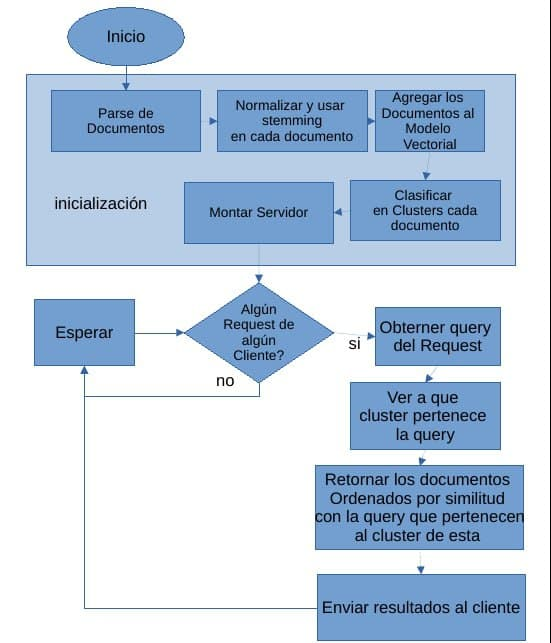
\includegraphics[width=0.5\textwidth]{img/diagram.jpg}
		\caption{Diagrama}
		\label{fig:diagram}
	\end{figure}
	
	
	\section{?`C\'omo esta estructurada la soluci\'on?} 
	%
	Existen dos proyectos que son dos aplicaciones diferentes, una utiliza los recursos que brinda la otra: 
	
	\subsection{Gugul Back}
	en esta soluci\'on es donde esta implementado el sistema. La estructura del proyecto est\'a distrubuida de la siguiente manera:
	
	\begin{verbatim}
	|-run.py
	|-documents.py
	|-document_handler.py
	|-test_collections
	|-collection_reader
	|-testers
	|-REARME.md
	|-requierments.txt
	
	\end{verbatim}
	
	\begin{flushleft}
		\begin{tabular}{@{}p{4cm}l}
			{\tt run.py}  & aplicaci\'on principal\\
			{\tt documents.py}  & representa los documentos para el corpus\\[2pt]
			{\tt document handler.py}& implementaci\'on del sistema\\[2pt]
			{\tt test collections}  & contiene las colecciones de prueba \\[2pt]
			{\tt collection reader}  & para manejar las colecciones \\[2pt]
			{\tt REARME.md}  & una descripcion y algunos aspectos de la soluci\'on \\[2pt]
			{\tt requirements.txt}& los requerimientos de la soluci\'on\\[2pt]			
			{\tt tester.py}  & para testear el sistema con las colecciones dadas\\
		\end{tabular}
	\end{flushleft}
	
	
	\paragraph{run.py} 
	Se encarga de brindar el servicio del lado del servidor de nuestra aplicaci\'on. Usa la libreria Flask de Python el cual nos permite en pocas lineas de c\'odigo lograr nuestro objetivo. Aqu\'i se crean las instancias de nuestro modelo vectorial.
	
	
	\paragraph{document.py}
	Es la definici\'on de un documento. Tiene un \textit{id} , \textit{title}, \textit{author} y \textit{texto}. Esto es lo que nos representa una instancia de un documento en esta  implementaci\'on
	
	\paragraph{document handler.py}
	Aqui hay una clase \textit{DocumentHandler.py} donde se encuentra la implementaci\'on del sistema. Esta implementaci\'on tiene una coleccion de documentos. A la hora de contruir el contenedor se llaman a varias funciones que inicializan y realizan parte del proceso de la recuperaci\'on , como tokenizar el texto y extraer las frecuencias para posteriores c\'alculos con las consultas que se hagan.
	
	\paragraph{test collections (folder)}
	Contiene las collecciones de prueba disponibles a usar en el motor de busqueda. Nosotros pusimos Cran y Med, el usuario final es libre de agregar m\'as.
	
	\paragraph{collection reader  (folder)} 
	Aqu\'i est\'an los encargados de retornar una lista con todos los documentos que contiene una colecci\'on espec\'ifica. La idea es que por cada colecci\'on haya un archivo dentro de esta carpeta que se encargue obtener la colecci\'on en Python a partir de las que se encuentren en la carpeta \textit{test collections}.
	
	
	\paragraph{testers (folder)} 
	Son los testers asociados a las colecciones que est\'en en \textit{test collections}, los cuales se deber\'ian de encargar de probar su colecci\'on asociada. Tienen por defecto pruebas con parametros que nos parecieron llamativos, si el usuario lo desea puede agregar a estos archivos pruebas con distintos par\'amentros del modelo vectorial.
	
	
	\paragraph{README.md} Aqu\'i  esta este documento con todo las partes de la implementaci\'on del sistema y algunas particularidades de esta soluci\'on.
	
	\paragraph{requerimets.txt}
	En `requirements.txt` estan los requerimientos de dependencias del proyecto que deben instalarse antes de que se corra la aplicaci\'on. el comando que debe correr se en el directorio del proyecto (es decir donde se encuentra el fichero \textit{requierements.txt}) es: \textit{pip install -r requirements.txt}
	
	
	
	
	
	
	
	\subsection{Gugul Front}
	
	
	\begin{flushleft}
		Esta aplicaci\'on corre en el navegador es un sitio web b\'asico implementado en \textbf{Vue} el cual es bastante amigable para el uso de nuestro sistema.
		\\
		Es una aplicaci\'on que corre en el navegador y hace pedidos a la aplicacion de gugul back para obtener los resultados del buscador y ser mostrados posteriormente al usuario en el navegador  
	\end{flushleft}
	
	\section{An\'alisis cr\'itico de las ventajas y desventajas del sistema desarrollado.}
	
	
	Se ha mostrado la arquitectura del modelo vectorial lo suficientemente abierto y flexible para ser usado en labores docentes, as\'i como investigaciones. La sencillez de esta arquitectura permitir\'a tanto la f\'acil observaci\'on de resultados y estructuras intermedias como la modificaci\'on y a\~nadido de nuevos m\'odulos y por tanto permite experimentar con el modelo. Puede ser usado en la docencia de algunas materias relacionadas directamente con la extracci\'on automatizada de informaci\'on.
	
	
	\subsection{Ventajas}
	Decidimos trabajar el modelo vectorial porque es un modelo que ha demostrado ser eficiente en SRI con repositorios grandes y de variadas tem\'aticas. En comparaci\'on con el modelo booleano es mejor para prop\'osito general, pues para booleano es recomendado que la informaci\'on que se trata de recolectar sea de un mismo tema, adem\'as de que es mas recomendable usar por expertos, no sucede asi con el vectorial, en cuyo caso puede ser usado facilmente por usuarios no expertos.
	
	para el desarrollo del modelo usamos el esquema de ponderaci\'on \textit{tf-idf} pues para los documentos este esquema mejora el rendimiento de la recuperaci\'on. La estrategia de coincidencia parcial que usa el modelo permite la recuperaci\'on de los documentos que mas se aproximen a los requerimientos de la consulta. La estrategia permite ordenar los documentos por orden de similitud con la consulta.
	
	\subsection{Desventajas}
	Un problema a resolver en el modelo es que  los t\'erminos indexados del documento son mutuamente independientes. Aunque en realidad existe relaci\'on entre algunos t\'erminos en el documento. Aunque podr\'ia significar una limitaci\'on del modelo simplifica el proceso de recuperaci\'on y en algunos casos mejora el rendimiento aunque a la hora de extracci\'on el proceso no sea tan abstracto como sistemas mas inteligantes. El an\'alisis de la correlacion requiere que se tangan enfoques mas avanzados en el sistema.
	
	Este modelo necesita de la intersecci\'on de los t\'erminos de la consulta con los documentos, en caso contrario no se produce la recuperaci\'on de informaci\'on
	
	Ademas al ser un modelo estad\'istico-matem\'atico, no tiene en cuenta la estructura sintáctico-semántica del lenguaje natural.
	
	%
	\section{Recomendaciones para trabajos futuros que mejoren la propuesta}
	
	 Se puede trabajar en el reconocimiento de entidades que ayuden a una mejor vinculaci\'on entre diferentes token de los documentos que guardan relaci\'on y pueden brindar mucha informaci\'on a la hora de determinar el peso de un documento en el \'ambito de la b\'usqueda . Tambi\'en se puede trabajar en correcciones b\'asicas como en interacciones con los usuarios que permitan al sistema saber que tan provechoso le fueron los resultado de la aplicaci\'on para una consulta dada, la informaci\'on recolectada se podr\'ia usar para pr\'oximas consultas similares o iguales. Se puede mejorar implementado algunas tecnicas para la retroalimentaci\'on, que es algo que podr\'ia ayudar al desempe\~no del sistema implementado aqu\'i 
	%
	
	
	\section*{Conslusiones} 
	
	Como pudo observarse en el desarrollo del sistema, las opciones que se toman en cada fase del roceso de extracci\'on de la informaci\'on puede influir en el resultado de la busqueda que de le sistema. Conseguir que exista una mezcla perfecta de las opciones en el trayecto de la recuperaci\'on de la informaci\'on es bastante dif\'icil , necesitaria horas y horas de evaluacion del sistema e implementaci\'on de mejoras. En el caso de Gugul, se puede concluir que a pesar de ser un sistema bastante sencillo que emplea el modelo vectorial, tiene resultados bastate satisfactorios. 
	
\end{document}
